\documentclass{article}%
\usepackage[T1]{fontenc}%
\usepackage[utf8]{inputenc}%
\usepackage{lmodern}%
\usepackage{textcomp}%
\usepackage{lastpage}%
\usepackage{parskip}%
\usepackage[top=4cm,hmargin=2cm,headheight=65pt,footskip=65pt]{geometry}%
\usepackage{amsmath}%
\usepackage{graphicx}%
\usepackage{needspace}%
\usepackage{color}%
\usepackage{longtable}%
\usepackage{multirow}%
\usepackage[table]{xcolor}%
\usepackage{fancyhdr}%
\usepackage{tabularx}%
%
\definecolor{OsdagGreen}{HTML}{D5DF93}%
\fancypagestyle{header}{ 
\renewcommand{\headrulewidth}{0pt}%
\renewcommand{\footrulewidth}{0pt}%
\fancyhead{ 
}%
\fancyfoot{ 
}%
\fancyhead[C]{ 
\begin{tabularx}{\textwidth}{|l|p{6cm}|l|X|}%
\hline%
\rowcolor{OsdagGreen}%
Company Name&&Project Title&\\%
\hline%
\rowcolor{OsdagGreen}%
Group/Team Name&&Subtitle&\\%
\hline%
\rowcolor{OsdagGreen}%
Designer&&Job Number&\\%
\hline%
\rowcolor{OsdagGreen}%
Date&05 /06 /2020&Client&\\%
\hline%
\end{tabularx}
}%
\fancyfoot[R]{ 
Page \thepage
}
}%
%
\begin{document}%
\normalsize%
\pagestyle{header}%
\section{Input Parameters}%
\label{sec:InputParameters}%
\renewcommand{\arraystretch}{1.2}%
\begin{longtable}{|p{5cm}|p{2cm}|p{2cm}|p{2cm}|p{5cm}|}%
\hline%
\hline%
\multicolumn{3}{|c|}{Module}&\multicolumn{2}{|c|}{Column Coverplate Connection}\\%
\hline%
\hline%
\multicolumn{3}{|c|}{MainModule}&\multicolumn{2}{|c|}{Moment Connection}\\%
\hline%
\hline%
\multicolumn{3}{|c|}{Moment(kNm)*}&\multicolumn{2}{|c|}{5.0}\\%
\hline%
\hline%
\multicolumn{3}{|c|}{Shear (kN)*}&\multicolumn{2}{|c|}{100.0}\\%
\hline%
\hline%
\multicolumn{3}{|c|}{Axial (kN) *}&\multicolumn{2}{|c|}{100.0}\\%
\hline%
\hline%
\multicolumn{5}{|c|}{\textbf{Section}}\\%
\hline%
\hline%
\multirow{11}{*}{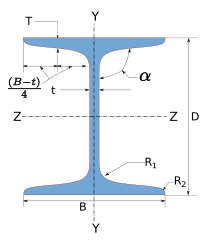
\includegraphics[width=5cm,height=5cm]{E:/office _anjali/columnspliceanjali/Osdag3/ResourceFiles/images/ISection.png}}&\multicolumn{2}{|c|}{Column Section *}&\multicolumn{2}{|c|}{UC 254 x 254 x 107}\\%
\cline{2%
-%
5}%
&\multicolumn{2}{|c|}{Material *}&\multicolumn{2}{|c|}{E 250 (Fe 410 W)A}\\%
\cline{2%
-%
5}%
&\multicolumn{2}{|c|}{Ultimate strength, fu (MPa)}&\multicolumn{2}{|c|}{410}\\%
\cline{2%
-%
5}%
&\multicolumn{2}{|c|}{Yield Strength , fy (MPa)}&\multicolumn{2}{|c|}{240}\\%
\cline{2%
-%
5}%
&Mass&107.1&R1(mm)&12.7\\%
\cline{2%
-%
5}%
&Area(mm2) {-} A&13640.0&R2(mm)&0.0\\%
\cline{2%
-%
5}%
&D(mm)&266.7&Iz(mm4)&175100000.0\\%
\cline{2%
-%
5}%
&B(mm)&258.8&Iy(mm4)&59270000.0\\%
\cline{2%
-%
5}%
&t(mm)&12.8&rz(mm)&113.0\\%
\cline{2%
-%
5}%
&T(mm)&20.5&ry(mm)&65.9\\%
\cline{2%
-%
5}%
&FlangeSlope&90&Zz(mm3)&1313000.0\\%
\cline{2%
-%
5}%
\hline%
\multicolumn{5}{|c|}{\textbf{Bolt Details}}\\%
\hline%
\hline%
\multicolumn{3}{|c|}{Preferences}&\multicolumn{2}{|c|}{Outside + Inside}\\%
\hline%
\hline%
\multicolumn{3}{|c|}{Diameter (mm)*}&\multicolumn{2}{|c|}{{[}12.0{]}}\\%
\hline%
\hline%
\multicolumn{3}{|c|}{Grade *}&\multicolumn{2}{|c|}{{[}3.6{]}}\\%
\hline%
\hline%
\multicolumn{3}{|c|}{Type *}&\multicolumn{2}{|c|}{Bearing Bolt}\\%
\hline%
\hline%
\multicolumn{3}{|c|}{Bolt hole type}&\multicolumn{2}{|c|}{Standard}\\%
\hline%
\hline%
\multicolumn{3}{|c|}{Slip factor (µ\_f)}&\multicolumn{2}{|c|}{0.3}\\%
\hline%
\hline%
\multicolumn{3}{|c|}{Type of edges}&\multicolumn{2}{|c|}{a {-} Sheared or hand flame cut}\\%
\hline%
\hline%
\multicolumn{3}{|c|}{Gap between beam and <br>support (mm)}&\multicolumn{2}{|c|}{10.0}\\%
\hline%
\hline%
\multicolumn{3}{|c|}{Are the members exposed to <br>corrosive influences}&\multicolumn{2}{|c|}{False}\\%
\hline%
\end{longtable}

%
\Needspace{10\baselineskip}%
\newpage%
\section{Design Checks}%
\label{sec:DesignChecks}%
\subsection{Member Capacity}%
\label{subsec:MemberCapacity}%
\renewcommand{\arraystretch}{1.2}%
\begin{longtable}{|p{4cm}|p{5cm}|p{5.5cm}|p{1.5cm}|}%
\hline%
\rowcolor{OsdagGreen}%
Check&Required&Provided&Remarks\\%
\hline%
\endhead%
\hline%
Axial Capacity Member (kN)&&$\begin{aligned} A_c &=\frac{A*f_y}{\gamma_{m0} *10^3}\\ &=\frac{13640.0*240}{1.1* 10^3}\\ &=2976.0\end{aligned}$&\\%
\hline%
Shear Capacity Member (kN)&&$\begin{aligned} S_c &= \frac{A_v*f_y}{\sqrt{3}*\gamma_{mo} *10^3}\\ &=\frac{225.7*12.8*240}{\sqrt{3}*1.1 *10^3}\\ &=363.91\end{aligned}$&\\%
\hline%
Plastic Moment Capacity (kNm)&&$\begin{aligned} Pmc &= \frac{\beta_b * Z_p *fy}{\gamma_{mo} * 10^6}\\ &=\frac{1*163009.57*240}{1.1 * 10^6}\\ &=35.57\end{aligned}$&\\%
\hline%
Moment Deformation Criteria (kNm)&&$\begin{aligned} Mdc &= \frac{1.5 *Z_e *fy}{1.1* 10^6}\\ &= \frac{1.5 *1313000.0*240}{1.1* 10^6}\\ &= 429.71\end{aligned}$&\\%
\hline%
Moment Capacity Member (kNm)&&$\begin{aligned} M_c &= min(Pmc,Mdc)\\ &=min(35.57,429.71)\\ &=35.57\end{aligned}$&\\%
\hline%
\end{longtable}

%
\newpage%
\subsection{Load Consideration}%
\label{subsec:LoadConsideration}%
\renewcommand{\arraystretch}{1.2}%
\begin{longtable}{|p{4cm}|p{3.5cm}|p{6.5cm}|p{1.5cm}|}%
\hline%
\rowcolor{OsdagGreen}%
Check&Required&Provided&Remarks\\%
\hline%
\endhead%
\hline%
Applied Axial Load (kN)&$\begin{aligned} Ac_{min} &= 0.3 * A_c\\ &= 0.3 *2976.0\\ &=892.8\\ Ac_{max} &= Ac \\ &=2976.0\end{aligned}$&$\begin{aligned} A_u &=892.8\end{aligned}$&Pass\\%
\hline%
Applied Shear Load (kN)&$\begin{aligned} Vc_{min} &= 0.6 * S_c\\ &= 0.6 *363.91\\ &=218.35\\ Vc_{max} &= Sc \\ &=363.91\end{aligned}$&$\begin{aligned} V_u &=218.35\end{aligned}$&Pass\\%
\hline%
Applied Moment Load (kNm)&$\begin{aligned} Mc_{min} &= 0.5 * M_c\\ &= 0.5 *35.57\\ &=17.78\\  Mc_{max} &= Mc \\ &=35.57\end{aligned}$&$\begin{aligned} M_u &=17.78\end{aligned}$&Pass\\%
\hline%
Forces Carried by Web&&$\begin{aligned}A_w &= Axial~ force~ in~ web  \\   &= \frac{(D- 2*T)*t* Au }{A} \\ &= \frac{(266.7- 2*20.5)*12.8*892.8 }{13640.0} \\ &=189.1~ kN\\ M_w &= Moment ~in ~web  \\  &= \frac{Z_w * Mu}{Z} \\ &= \frac{163009.57 * 17.78}{1484000.0} \\ &=1.95~{kNm}\end{aligned}$&\\%
\hline%
Forces Carried by Flange&&$\begin{aligned} A_f&= Axial~force~ in ~flange  \\ &= \frac{Au * B *T}{A} \\ &= \frac{892.8 * 258.8*20.5}{13640.0} \\ &=347.26~ kN\\ M_f& =Moment~ in~ flange \\  & = Mu-M_w\\ &= 17.78-1.95\\ &=15.83~{kNm}\\  F_f& =flange~force  \\ & = \frac{M_f *10^3}{D-T} + A_f \\ &= \frac{15.83* 10^3}{266.7-20.5} +347.26 \\ &=411.56~kN \end{aligned}$&\\%
\hline%
\end{longtable}

%
\newpage%
\subsection{Initial Member Check}%
\label{subsec:InitialMemberCheck}%
\renewcommand{\arraystretch}{1.2}%
\begin{longtable}{|p{3cm}|p{4.5cm}|p{6.5cm}|p{1.5cm}|}%
\hline%
\rowcolor{OsdagGreen}%
Check&Required&Provided&Remarks\\%
\hline%
\endhead%
\hline%
Tension Yielding Capacity (kN)&$\begin{aligned} F_f &=411.56\end{aligned}$&$\begin{aligned} T_{dg} &= \frac{l*t*f_y}{\gamma_{mo}}\\ &=\frac{1*258.8*20.5*240}{1.1}\\ &=1205.77\end{aligned}$&Pass\\%
\hline%
Web Tension Yielding Capacity (kN)&$\begin{aligned} A_w &=189.1\end{aligned}$&$\begin{aligned} T_{dg} &= \frac{l*t*f_y}{\gamma_{mo}}\\ &=\frac{1*225.7*12.8*240}{1.1}\\ &=657\end{aligned}$&Pass\\%
\hline%
\end{longtable}

%
\newpage%
\subsection{Initial flange plate height check}%
\label{subsec:Initialflangeplateheightcheck}%
\renewcommand{\arraystretch}{1.2}%
\begin{longtable}{|p{4.5cm}|p{2.5cm}|p{7cm}|p{1.5cm}|}%
\hline%
\rowcolor{OsdagGreen}%
Check&Required&Provided&Remarks\\%
\hline%
\endhead%
\hline%
Flange\_Plate.Height&Bfp >= 50&$\begin{aligned} B_{fp} &=258.8\end{aligned}$&Pass\\%
\hline%
Flange\_Plate.InnerHeight&Bifp >= 50&$\begin{aligned} B_{fp} &= \frac{B-t-(2*R1)}{2}\\ &=\frac{258.8-12.8-(2*12.7)}{2}\\ &= 110.3\end{aligned}$&Pass\\%
\hline%
\end{longtable}

%
\newpage%
\subsection{Flange plate thickness}%
\label{subsec:Flangeplatethickness}%
\renewcommand{\arraystretch}{1.2}%
\begin{longtable}{|p{2.5cm}|p{5cm}|p{6.5cm}|p{1.5cm}|}%
\hline%
\rowcolor{OsdagGreen}%
Check&Required&Provided&Remarks\\%
\hline%
\endhead%
\hline%
Thickness (mm)*&$\begin{aligned} T &=10.25\end{aligned}$&$\begin{aligned} t_{fp} &=12.0\end{aligned}$&Pass\\%
\hline%
Plate Area check (mm2)&$\begin{aligned} &pt.area >= \\&connected~member~area * 1.05\\  &= 5570.67\end{aligned}$&$\begin{aligned} B_{fp} &= B\\ &= 258.8 \\ B_{ifp} &= \frac{B-t-(2*R1)}{2}\\ &=\frac{258.8-12.8-(2*12.7)}{2}\\ &= 110.3 \\  pt.area &=(258.8+(2*110.3))*12.0\\ &= 5752.8\end{aligned}$&Pass\\%
\hline%
\end{longtable}

%
\newpage%
\subsection{Initial web plate height check}%
\label{subsec:Initialwebplateheightcheck}%
\renewcommand{\arraystretch}{1.2}%
\begin{longtable}{|p{4.5cm}|p{2.5cm}|p{7cm}|p{1.5cm}|}%
\hline%
\rowcolor{OsdagGreen}%
Check&Required&Provided&Remarks\\%
\hline%
\endhead%
\hline%
Web\_Plate.Height&$\begin{aligned}  &= 0.6 *D\\  &= 0.6 *266.7\\  &= 160.02\end{aligned}$&$\begin{aligned} C~~ &= max((R1, t_{ifp}) + 10) \\ &= max((12.7,12.0) +10) \\ &= 22.7 \\  W_{wp} &= D - (2 * T) - (2 * C)\\  &= 266.7 - (2 * 20.5) - (2 *22.7)\\  &=180.3\end{aligned}$&Pass\\%
\hline%
\end{longtable}

%
\newpage%
\subsection{Web plate thickness}%
\label{subsec:Webplatethickness}%
\renewcommand{\arraystretch}{1.2}%
\begin{longtable}{|p{2.5cm}|p{5cm}|p{6.5cm}|p{1.5cm}|}%
\hline%
\rowcolor{OsdagGreen}%
Check&Required&Provided&Remarks\\%
\hline%
\endhead%
\hline%
Thickness (mm)*&$\begin{aligned} t &=6.4\end{aligned}$&$\begin{aligned} t_{wp} &=10.0\end{aligned}$&Pass\\%
\hline%
Plate Area check (mm2)&$\begin{aligned} &pt.area >= \\&connected~member~area * 1.05\\  &= 3033.41\end{aligned}$&$\begin{aligned}pt.area &= t_{wp} *2*  W_{wp} \\ &= 10.0*2* 180.3\\ &= 3606.0\end{aligned}$&Pass\\%
\hline%
\end{longtable}

%
\newpage%
\subsection{Web Spacing Checks}%
\label{subsec:WebSpacingChecks}%
\renewcommand{\arraystretch}{1.2}%
\begin{longtable}{|p{2.5cm}|p{7.5cm}|p{5cm}|p{1cm}|}%
\hline%
\rowcolor{OsdagGreen}%
Check&Required&Provided&Remarks\\%
\hline%
\endhead%
\hline%
Min.Diameter (mm)&&$\begin{aligned} d &=12.0\end{aligned}$&\\%
\hline%
Min. Gauge (mm)&$\begin{aligned}p/g_{min}&= 2.5 ~ d&\\ =&2.5*12.0&=30.0\end{aligned}$&$\begin{aligned} g &=30~(Col~Limit~(c_l) = 2)\end{aligned}$&\\%
\hline%
Min. Edge Distance (mm)&$\begin{aligned}e/e`_{min} &=[1.5~or~ 1.7] * d_0\\ &=1.7*13.0=22.1 \end{aligned}$&25&\\%
\hline%
Spacing Check&$\begin{aligned} depth & = 2 * e + (c_l -1) * g\\ & = 2 * 25+(2.0-1)*30\\ & = 80.0\end{aligned}$&180.3&Pass\\%
\hline%
\end{longtable}

%
\newpage%
\subsection{Flange Spacing Checks}%
\label{subsec:FlangeSpacingChecks}%
\renewcommand{\arraystretch}{1.2}%
\begin{longtable}{|p{2.5cm}|p{7.5cm}|p{5cm}|p{1cm}|}%
\hline%
\rowcolor{OsdagGreen}%
Check&Required&Provided&Remarks\\%
\hline%
\endhead%
\hline%
Min.Diameter (mm)&&$\begin{aligned} d &=12.0\end{aligned}$&\\%
\hline%
Min. Gauge (mm)&$\begin{aligned}p/g_{min}&= 2.5 ~ d&\\ =&2.5*12.0&=30.0\end{aligned}$&$\begin{aligned} g &=0.0~(Col~Limit~(c_l) = 1)\end{aligned}$&\\%
\hline%
Min. Edge Distance (mm)&$\begin{aligned}e/e`_{min} &=[1.5~or~ 1.7] * d_0\\ &=1.7*13.0=22.1 \end{aligned}$&25&\\%
\hline%
Spacing Check&$\begin{aligned} depth & = 2 * e + (c_l -1) * g\\ & = 2 * 25+(1.0-1)*30\\ & = 50.0\end{aligned}$&110.3&Pass\\%
\hline%
\end{longtable}

%
\newpage%
\subsection{Flange Bolt Checks}%
\label{subsec:FlangeBoltChecks}%
\renewcommand{\arraystretch}{1.2}%
\begin{longtable}{|p{3cm}|p{5.5cm}|p{6cm}|p{1.5cm}|}%
\hline%
\rowcolor{OsdagGreen}%
Check&Required&Provided&Remarks\\%
\hline%
\endhead%
\hline%
Diameter (mm)&Bolt Quantity Optimisation&$\begin{aligned} d &=12.0\end{aligned}$&\\%
\hline%
Grade&Bolt Grade Optimisation&3.6&\\%
\hline%
Bolt Ultimate Strength (N/mm2)&&$\begin{aligned} f_{ub} &=330.0\end{aligned}$&\\%
\hline%
Bolt Yield Strength (N/mm2)&&$\begin{aligned} f_{yb} &=190.0\end{aligned}$&\\%
\hline%
Nominal Stress Area (mm2)& &$\begin{aligned} A_{nb} &=84.3~( Ref~IS~1367-3~(2002))\end{aligned}$&\\%
\hline%
Hole Diameter (mm)& &$\begin{aligned} d_0 &=13.0\end{aligned}$&\\%
\hline%
Shear Capacity (kN)&&$\begin{aligned}V_{dsb} &= \frac{f_{ub} ~n_n~ A_{nb}}{\sqrt{3} ~\gamma_{mb}}\\ &= \frac{330.0*2*84.3}{\sqrt{3}~*~1.25}\\ &= 25.7\end{aligned}$&\\%
\hline%
Bearing Capacity (kN)&&$\begin{aligned}V_{dpb} &= \frac{2.5~ k_b~ d~ t~ f_u}{\gamma_{mb}}\\ &= \frac{2.5~*0.52*12.0*20.5*410}{1.25}\\ &=104.89\end{aligned}$&\\%
\hline%
Bolt Capacity (kN)&&$\begin{aligned}V_{db} &= min~ (V_{dsb}, V_{dpb})\\ &= min~ (25.7,104.89)\\ &=25.7\end{aligned}$&\\%
\hline%
No of Bolts&$\begin{aligned}R_{u} &= \sqrt{V_u^2+A_u^2}\\ n_{trial} &= R_u/ V_{bolt}\\ R_{u} &= \frac{2*\sqrt{0.0^2+411.56^2}}{25.7}\\ &=34\end{aligned}$&36&\\%
\hline%
No of Columns&&$\begin{aligned} n_c &=6\end{aligned}$&\\%
\hline%
No of Rows&&$\begin{aligned} n_r &=6\end{aligned}$&\\%
\hline%
Min. Pitch (mm)&$\begin{aligned}p/g_{min}&= 2.5 ~ d&\\ =&2.5*12.0&=30.0\end{aligned}$&30&Pass\\%
\hline%
Max. Pitch (mm)&$\begin{aligned}p/g_{max} &=\min(32~t,~300~mm)&\\ &=\min(32 *~12.0,~ 300 ~mm)\\&=300\\  t& = min(12.0,12.0)\end{aligned}$&30&Pass\\%
\hline%
Min. Gauge (mm)&$\begin{aligned}p/g_{min}&= 2.5 ~ d&\\ =&2.5*12.0&=30.0\end{aligned}$&30&Pass\\%
\hline%
Max. Gauge (mm)&$\begin{aligned}p/g_{max} &=\min(32~t,~300~mm)&\\ &=\min(32 *~12.0,~ 300 ~mm)\\&=300\\  t& = min(12.0,12.0)\end{aligned}$&30&Pass\\%
\hline%
Min. End Distance (mm)&$\begin{aligned}e/e`_{min} &=[1.5~or~ 1.7] * d_0\\ &=1.7*13.0=22.1 \end{aligned}$&25&Pass\\%
\hline%
Max. End Distance (mm)&$\begin{aligned}e/e`_{max} &= 12~ t~ \varepsilon&\\ \varepsilon &= \sqrt{\frac{250}{f_y}}\\ e/e`_{max}&=12 ~*12.0*\sqrt{\frac{250}{250}}\\ &=144.0\\ \end{aligned}$&25&Pass\\%
\hline%
Min. Edge Distance (mm)&$\begin{aligned}e/e`_{min} &=[1.5~or~ 1.7] * d_0\\ &=1.7*13.0=22.1 \end{aligned}$&25.15&Pass\\%
\hline%
Max. Edge Distance (mm)&$\begin{aligned}e/e`_{max} &= 12~ t~ \varepsilon&\\ \varepsilon &= \sqrt{\frac{250}{f_y}}\\ e/e`_{max}&=12 ~*12.0*\sqrt{\frac{250}{250}}\\ &=144.0\\ \end{aligned}$&25.15&Pass\\%
\hline%
Bolt Capacity post Long Joint (kN)&$\begin{aligned} &if~l\geq 15 * d~then~V_{rd} = \beta_{ij} * V_{db} \\ & if~l < 15 * d~then~V_{rd} = V_{db} \\ & where,\\ & l = ((nc~or~nr) - 1) * (p~or~g) \\ & \beta_{ij} = 1.075 - l/(200 * d) \\ & but~0.75\leq\beta_{ij}\leq1.0 \end{aligned}$&$\begin{aligned} l~&= ((nc~or~nr) - 1) * (p~or~g) \\  lc&= 2*((\frac{6}{2} - 1) * 30+25)+ 10.0\\&=180.0\\  lr&= 2*((\frac{6}{2} - 1) * 30+25.15\\& +12.7)+ 12.8=208.5\\  l~&= 208.5\\ &15 * d = 15 * 12.0 = 180.0 \\ &since,~l \geq 15 * d~\\ &then~V_{rd} = \beta_{ij} * V_{db} \\ \beta_{ij} &= 1.075 - 208.5/(200*12.0)\\& =0.99\\  V_{rd}& = 0.99 * 25.7=25.7 \end{aligned}$&\\%
\hline%
Capacity (kN)&22.86&25.7&Pass\\%
\hline%
\end{longtable}

%
\newpage%
\subsection{Web Bolt Checks}%
\label{subsec:WebBoltChecks}%
\renewcommand{\arraystretch}{1.2}%
\begin{longtable}{|p{3cm}|p{5cm}|p{7.5cm}|p{1.5cm}|}%
\hline%
\rowcolor{OsdagGreen}%
Check&Required&Provided&Remarks\\%
\hline%
\endhead%
\hline%
Shear Capacity (kN)&&$\begin{aligned}V_{dsb} &= \frac{f_{ub} ~n_n~ A_{nb}}{\sqrt{3} ~\gamma_{mb}}\\ &= \frac{330.0*2*84.3}{\sqrt{3}~*~1.25}\\ &= 25.7\end{aligned}$&\\%
\hline%
Bearing Capacity (kN)&&$\begin{aligned}V_{dpb} &= \frac{2.5~ k_b~ d~ t~ f_u}{\gamma_{mb}}\\ &= \frac{2.5~*0.52*12.0*12.8*410}{1.25}\\ &=65.5\end{aligned}$&\\%
\hline%
Bolt Capacity (kN)&&$\begin{aligned}V_{db} &= min~ (V_{dsb}, V_{dpb})\\ &= min~ (25.7,65.5)\\ &=25.7\end{aligned}$&\\%
\hline%
No of Bolts&$\begin{aligned}R_{u} &= \sqrt{V_u^2+A_u^2}\\ n_{trial} &= R_u/ V_{bolt}\\ R_{u} &= \frac{2*\sqrt{218.35^2+189.1^2}}{25.7}\\ &=24\end{aligned}$&150&\\%
\hline%
No of Rows&&$\begin{aligned} n_r &=30\end{aligned}$&\\%
\hline%
No of Columns&&$\begin{aligned} n_c &=5\end{aligned}$&\\%
\hline%
Min. Pitch (mm)&$\begin{aligned}p/g_{min}&= 2.5 ~ d&\\ =&2.5*12.0&=30.0\end{aligned}$&30&Pass\\%
\hline%
Max. Pitch (mm)&$\begin{aligned}p/g_{max} &=\min(32~t,~300~mm)&\\ &=\min(32 *~10.0,~ 300 ~mm)\\&=300\\  t& = min(10.0,10.0)\end{aligned}$&30&Pass\\%
\hline%
Min. Gauge (mm)&$\begin{aligned}p/g_{min}&= 2.5 ~ d&\\ =&2.5*12.0&=30.0\end{aligned}$&30&Pass\\%
\hline%
Max. Gauge (mm)&$\begin{aligned}p/g_{max} &=\min(32~t,~300~mm)&\\ &=\min(32 *~10.0,~ 300 ~mm)\\&=300\\  t& = min(10.0,10.0)\end{aligned}$&30&Pass\\%
\hline%
Min. End Distance (mm)&$\begin{aligned}e/e`_{min} &=[1.5~or~ 1.7] * d_0\\ &=1.7*13.0=22.1 \end{aligned}$&25&Pass\\%
\hline%
Max. End Distance (mm)&$\begin{aligned}e/e`_{max} &= 12~ t~ \varepsilon&\\ \varepsilon &= \sqrt{\frac{250}{f_y}}\\ e/e`_{max}&=12 ~*10.0*\sqrt{\frac{250}{250}}\\ &=120.0\\ \end{aligned}$&25&Pass\\%
\hline%
Min. Edge Distance (mm)&$\begin{aligned}e/e`_{min} &=[1.5~or~ 1.7] * d_0\\ &=1.7*13.0=22.1 \end{aligned}$&25&Pass\\%
\hline%
Max. Edge Distance (mm)&$\begin{aligned}e/e`_{max} &= 12~ t~ \varepsilon&\\ \varepsilon &= \sqrt{\frac{250}{f_y}}\\ e/e`_{max}&=12 ~*10.0*\sqrt{\frac{250}{250}}\\ &=120.0\\ \end{aligned}$&25&Pass\\%
\hline%
Parameters required for bolt force (mm)&&$\begin{aligned} l_n~~~ &= length~available \\  l_n~~~ &= g * (n_c - 1)\\  &= 30 * (5 - 1)\\  & =120\\  y_{max} &= l_n / 2\\  &= 120 / 2 \\  & =60.0\\ x_{max} &= p * (\frac{n_r}{2} - 1) / 2 \\  &= 30 * (\frac{30}{2} - 1) / 2 \\  & =210.0\end{aligned}$&\\%
\hline%
Moment Demand (kNm&&$\begin{aligned}  M_d &= (V_u * ecc + M_w)\\  &= \frac{(218.35 * 10^3 *435.0 + 1.95*10^6)}{10^6}\\  & =96.94\end{aligned}$&\\%
\hline%
Bolt.Force&&$\begin{aligned} vbv~~ &= V_u / ((n_r/2) * n_c)\\  &= \frac{218.35}{ (5*(30/2))}\\  & =2.91\\ tmh~ &= \frac{M_d * y_{max} }{ \Sigma r_i^2} \\  &= \frac{96.94 *60.0}{1395.0}\\  & =4.17\\  tmv ~&= \frac{M_d * x_{max}}{\Sigma r_i^2}\\ &= \frac{96.94 * 210.0}{1395.0}\\  & =14.59\\  abh~ & = \frac{A_u }{((n_r/2) * n_c)}\\   & =\frac{189.1}{ (5 *(30/2))}\\  & =2.52\\  vres &=\sqrt{(vbv +tmv) ^ 2 + (tmh+abh) ^ 2}\\   &= \sqrt{(2.91 +14.59) ^2 + (4.17+2.52) ^ 2}\\  & =18.74\end{aligned}$&\\%
\hline%
Bolt Capacity post Long Joint (kN)&$\begin{aligned} &if~l\geq 15 * d~then~V_{rd} = \beta_{ij} * V_{db} \\ & if~l < 15 * d~then~V_{rd} = V_{db} \\ & where,\\ & l = ((nc~or~nr) - 1) * (p~or~g) \\ & \beta_{ij} = 1.075 - l/(200 * d) \\ & but~0.75\leq\beta_{ij}\leq1.0 \end{aligned}$&$\begin{aligned} l&= ((nc~or~nr) - 1) * (p~or~g) \\  lc&= 2*((\frac{30}{2} - 1) * 30+25)+ 10.0\\&=900.0\\  lr&= (5 - 1) * 30=120\\  l&= 900.0\\ & 15 * d = 15 * 12.0 = 180.0 \\ &since,~l \geq 15 * d~ \\&then~V_{rd} = \beta_{ij} * V_{db} \\ \beta_{ij} &= 1.075 - 900.0/(200*12.0) \\&=0.75\\ V_{rd} &= 0.75 * 25.7=19.27 \end{aligned}$&\\%
\hline%
Capacity (kN)&18.74&19.27&Pass\\%
\hline%
\end{longtable}

%
\newpage%
\subsection{Inner and Outer flange plate Checks}%
\label{subsec:InnerandOuterflangeplateChecks}%
\renewcommand{\arraystretch}{1.2}%
\begin{longtable}{|p{4cm}|p{6cm}|p{5.5cm}|p{1.5cm}|}%
\hline%
\rowcolor{OsdagGreen}%
Check&Required&Provided&Remarks\\%
\hline%
\endhead%
\hline%
Min. Plate Height (mm)&$\begin{aligned}min~flange~plate~ht &= beam~width\\ &=258.8\end{aligned}$&258.8&Pass\\%
\hline%
Min. Plate Length (mm)&$\begin{aligned} & 2[2*e_{min} + ({\frac{n_r}{2}}-1) * p_{min})]\\ & +\frac{gap}{2}]\\ &=2*[(2*22.1 + (\frac{6}{2}-1) * 30.0\\ &= + \frac{10.0}{2}]\\ &=218.4\end{aligned}$&230.0&Pass\\%
\hline%
Min. Inner Plate Height (mm)&$\begin{aligned}&= \frac{B -t- (2*R1)}{2}\\ &=\frac{258.8 -12.8 - 2*12.7}{2}\\ &=110\end{aligned}$&110&Pass\\%
\hline%
Max. Inner Plate Height (mm)&$\begin{aligned}&= \frac{B -t- (2*R1)}{2}\\ &=\frac{258.8 -12.8 - 2*12.7}{2}\\ &=110\end{aligned}$&110&Pass\\%
\hline%
Min. Inner Plate Length (mm)&$\begin{aligned} & 2[2*e_{min} + ({\frac{n_r}{2}}-1) * p_{min})]\\ & +\frac{gap}{2}]\\ &=2*[(2*22.1 + (\frac{6}{2}-1) * 30.0\\ &= + \frac{10.0}{2}]\\ &=218.4\end{aligned}$&230.0&Pass\\%
\hline%
Min.Plate Thickness (mm)&$\begin{aligned} T/2 &=10.25\end{aligned}$&$\begin{aligned} t_{ifp} &=12.0\end{aligned}$&Pass\\%
\hline%
\end{longtable}

%
\newpage%
\subsection{Web Plate Rechecks}%
\label{subsec:WebPlateRechecks}%
\renewcommand{\arraystretch}{1.2}%
\begin{longtable}{|p{4cm}|p{6cm}|p{5.5cm}|p{1.5cm}|}%
\hline%
\rowcolor{OsdagGreen}%
Check&Required&Provided&Remarks\\%
\hline%
\endhead%
\hline%
Min. Plate Height (mm)&$\begin{aligned}  &= 0.6 *D\\  &= 0.6 *266.7\\  &= 160.02\end{aligned}$&170&Pass\\%
\hline%
Min. Plate Length (mm)&$\begin{aligned} & 2[2*e_{min} + ({\frac{n_r}{2}}-1) * p_{min})]\\ & +\frac{gap}{2}]\\ &=2*[(2*22.1 + (\frac{30}{2}-1) * 30.0\\ &= + \frac{10.0}{2}]\\ &=938.4\end{aligned}$&950.0&Pass\\%
\hline%
Min.Plate Thickness (mm)&$\begin{aligned} t/2 &=6.4\end{aligned}$&$\begin{aligned} t_{wp} &=10.0\end{aligned}$&Pass\\%
\hline%
\end{longtable}

%
\newpage%
\subsection{Member Checks}%
\label{subsec:MemberChecks}%
\renewcommand{\arraystretch}{1.2}%
\begin{longtable}{|p{4cm}|p{4cm}|p{7cm}|p{1.5cm}|}%
\hline%
\rowcolor{OsdagGreen}%
Check&Required&Provided&Remarks\\%
\hline%
\endhead%
\hline%
Tension Yielding Capacity (kN)&&$\begin{aligned} T_{dg} &= \frac{l*t*f_y}{\gamma_{mo}}\\ &=\frac{1*258.8*20.5*240}{1.1}\\ &=1205.77\end{aligned}$&\\%
\hline%
Tension Rupture Capacity (kN)&&$\begin{aligned} T_{dn} &= \frac{0.9*A_{n}*f_u}{\gamma_{m1}}\\ &=\frac{1*0.9* (258.8-6*13.0)*20.5*410}{1.25}\\ &=1094.13\end{aligned}$&\\%
\hline%
Block Shear Capacity (kN)&&$\begin{aligned}T_{db1} &= \frac{A_{vg} f_{y}}{\sqrt{3} \gamma_{m0}} + \frac{0.9 A_{tn} f_{u}}{\gamma_{m1}}\\ T_{db2} &= \frac{0.9*A_{vn} f_{u}}{\sqrt{3} \gamma_{m1}} + \frac{A_{tg} f_{y}}{\gamma_{m0}}\\ T_{db} &= min(T_{db1}, T_{db2})= 1094.52\end{aligned}$&\\%
\hline%
Flange Tension Capacity (kN)&$\begin{aligned} F_f &=411.56\end{aligned}$&$\begin{aligned} T_d &= min(T_{dg},T_{dn},T_{db})\\ &= min(1205.77,1094.13,1094.52)\\ &=1094.13\end{aligned}$&Pass\\%
\hline%
Web Tension Yielding Capacity (kN)&&$\begin{aligned} T_{dg} &= \frac{l*t*f_y}{\gamma_{mo}}\\ &=\frac{1*225.7*12.8*240}{1.1}\\ &=656.58\end{aligned}$&\\%
\hline%
Web Tension Rupture Capacity (kN)&&$\begin{aligned} T_{dn} &= \frac{0.9*A_{n}*f_u}{\gamma_{m1}}\\ &=\frac{1*0.9* (225.7-5*13.0)*12.8*410}{1.25}\\ &=607.21\end{aligned}$&\\%
\hline%
Block Shear Capacity (kN)&&$\begin{aligned}T_{db1} &= \frac{A_{vg} f_{y}}{\sqrt{3} \gamma_{m0}} + \frac{0.9 A_{tn} f_{u}}{\gamma_{m1}}\\ T_{db2} &= \frac{0.9*A_{vn} f_{u}}{\sqrt{3} \gamma_{m1}} + \frac{A_{tg} f_{y}}{\gamma_{m0}}\\ T_{db} &= min(T_{db1}, T_{db2})= 1846.22\end{aligned}$&\\%
\hline%
Web Tension Capacity (kN)&$\begin{aligned} A_w &=189.1\end{aligned}$&$\begin{aligned} T_d &= min(T_{dg},T_{dn},T_{db})\\ &= min(656.58,607.21,1846.22)\\ &=607.21\end{aligned}$&Pass\\%
\hline%
\end{longtable}

%
\newpage%
\subsection{Flange Plate Capacity Checks in axial{-}Outside/Inside }%
\label{subsec:FlangePlateCapacityChecksinaxial{-}Outside/Inside}%
\renewcommand{\arraystretch}{1.2}%
\begin{longtable}{|p{4cm}|p{4cm}|p{7cm}|p{1.5cm}|}%
\hline%
\rowcolor{OsdagGreen}%
Check&Required&Provided&Remarks\\%
\hline%
\endhead%
\hline%
Tension Yielding Capacity (kN)&&$\begin{aligned} T_{dg} &= \frac{l*t*f_y}{\gamma_{mo}}\\ &=\frac{1*478.8*12.0*250}{1.1}\\ &=1305.82\end{aligned}$&\\%
\hline%
Tension Rupture Capacity (kN)&&$\begin{aligned} T_{dn} &= \frac{0.9*A_{n}*f_u}{\gamma_{m1}}\\ &=\frac{1*0.9* (478.8-6*13.0)*12.0*410}{1.25}\\ &=1419.79\end{aligned}$&\\%
\hline%
Block Shear Capacity (kN)&&$\begin{aligned}T_{db1} &= \frac{A_{vg} f_{y}}{\sqrt{3} \gamma_{m0}} + \frac{0.9 A_{tn} f_{u}}{\gamma_{m1}}\\ T_{db2} &= \frac{0.9*A_{vn} f_{u}}{\sqrt{3} \gamma_{m1}} + \frac{A_{tg} f_{y}}{\gamma_{m0}}\\ T_{db} &= min(T_{db1}, T_{db2})= 1416.71\end{aligned}$&\\%
\hline%
Plate Tension Capacity (kN)&$\begin{aligned} F_f &=411.56\end{aligned}$&$\begin{aligned} T_d &= min(T_{dg},T_{dn},T_{db})\\ &= min(1305.82,1419.79,1416.71)\\ &=1305.82\end{aligned}$&Pass\\%
\hline%
\end{longtable}

%
\newpage%
\subsection{Web Plate Capacity Checks in Axial}%
\label{subsec:WebPlateCapacityChecksinAxial}%
\renewcommand{\arraystretch}{1.2}%
\begin{longtable}{|p{4cm}|p{4cm}|p{7cm}|p{1.5cm}|}%
\hline%
\rowcolor{OsdagGreen}%
Check&Required&Provided&Remarks\\%
\hline%
\endhead%
\hline%
Tension Yielding Capacity (kN)&&$\begin{aligned} T_{dg} &= \frac{l*t*f_y}{\gamma_{mo}}\\ &=\frac{2*170*10.0*250}{1.1}\\ &=772.73\end{aligned}$&\\%
\hline%
Tension Rupture Capacity (kN)&&$\begin{aligned} T_{dn} &= \frac{0.9*A_{n}*f_u}{\gamma_{m1}}\\ &=\frac{2*0.9* (170-5*13.0)*10.0*410}{1.25}\\ &=619.92\end{aligned}$&\\%
\hline%
Block Shear Capacity (kN)&&$\begin{aligned}T_{db1} &= \frac{A_{vg} f_{y}}{\sqrt{3} \gamma_{m0}} + \frac{0.9 A_{tn} f_{u}}{\gamma_{m1}}\\ T_{db2} &= \frac{0.9*A_{vn} f_{u}}{\sqrt{3} \gamma_{m1}} + \frac{A_{tg} f_{y}}{\gamma_{m0}}\\ T_{db} &= min(T_{db1}, T_{db2})= 2884.72\end{aligned}$&\\%
\hline%
Web Plate Tension Capacity (kN)&$\begin{aligned} A_w &=189.1\end{aligned}$&$\begin{aligned} T_d &= min(T_{dg},T_{dn},T_{db})\\ &= min(772.73,619.92,2884.72)\\ &=619.92\end{aligned}$&Pass\\%
\hline%
\end{longtable}

%
\newpage%
\subsection{Web Plate Capacity Checks in Shear}%
\label{subsec:WebPlateCapacityChecksinShear}%
\renewcommand{\arraystretch}{1.2}%
\begin{longtable}{|p{4cm}|p{4cm}|p{7cm}|p{1.5cm}|}%
\hline%
\rowcolor{OsdagGreen}%
Check&Required&Provided&Remarks\\%
\hline%
\endhead%
\hline%
Shear Yielding Capacity (kN)&&$\begin{aligned} V_{dy} &= \frac{A_v*f_y}{\sqrt{3}*\gamma_{mo}}\\ &=\frac{2*170*10.0*250}{\sqrt{3}*1.1}\\ &=446.13\end{aligned}$&\\%
\hline%
Shear Rupture Capacity (kN)&&$\begin{aligned} V_{dn} &= \frac{0.9*A_{vn}*f_u}{\sqrt{3}*\gamma_{m1}}\\ &= \frac{2*0.9 *(170-(5*13.0))*10.0*410}{\sqrt{3}*1.25}\\ &=357.91\end{aligned}$&\\%
\hline%
Block Shear Capacity (kN)&&$\begin{aligned}V_{db1} &= \frac{A_{vg} f_{y}}{\sqrt{3} \gamma_{m0}} + \frac{0.9 A_{tn} f_{u}}{\gamma_{m1}}\\ V_{db2} &= \frac{0.9*A_{vn} f_{u}}{\sqrt{3} \gamma_{m1}} + \frac{A_{tg} f_{y}}{\gamma_{m0}}\\ V_{db} &= min(V_{db1}, V_{db2})= 2317.58\end{aligned}$&\\%
\hline%
Web Plate Shear Capacity (kN)&$\begin{aligned} V_u &=218.35\end{aligned}$&$\begin{aligned} V_d &= min(V_{dy},V_{dn},V_{db})\\ &= min(446.13,357.91,2317.58)\\ &=357.91\end{aligned}$&Pass\\%
\hline%
\end{longtable}

%
\Needspace{10\baselineskip}%
\newpage%
\end{document}